\section{Mollification of sets of least perimeter}\label{MollifierSection}
In this section our goal is to show that given a set $U$ of least perimeter, we can find a $C^1$ hypersurface $N$ which approximates $\partial^* U$ arbitrarily well.
As in the prequel we assume that $g$ has uniformly negative Ricci curvature; we fix an ``origin'' $O \in M$, $\delta > 0$, and normal coordinates $(x^\mu)$ in $B_\delta := B(O, \delta)$.
Then the difference $P - Q$ of two points will be taken with respect to the normal coordinates, and we write $\Phi(r, \theta)$ for the point with polar coordinates $(r, \theta)$ where the polar coordinates are induced by $(x^\mu)$.
We also recall the definition of the closed $d-1$-form $\psi$ given by (\ref{d1 form}).

\begin{proposition}\label{mollifier quant}
For every $\varepsilon > 0$ there exists $\gamma^* > 0$ such that for every set $U$ of least perimeter $B_\delta$, such that
\begin{equation}\label{bootstrap the mollifier}
\gamma := \delta^{1 - d}\int_{B_\delta} *|\dif 1_U| - \dif 1_U \wedge \psi < \gamma^*,
\end{equation}
and almost every $t \in (0, \delta)$, there exists a set $V$ of $C^1$ perimeter in $B_t$, such that
\begin{align}
|V \cap B_t| &\leq \eta(V, B_t) + \varepsilon \delta^{d - 1} \gamma, \label{mollifier quant1}\\
\left||U \cap B_t| - |V \cap B_t|\right| &\leq \varepsilon \delta^{d - 1} \gamma, \label{mollifier quant2}\\
(\normal_V, \psi/|\psi|) &\geq (1 - \varepsilon) \text{ on } B_{t-\varepsilon}, \label{mollifier quant4}
\end{align}
and for every vector field $Y$ defined near $P$ with $|Y| \sim 1$ and $|\Div Y| \lesssim 1$,
\begin{equation}
\left|\int_{B_t} *Y(1_U - 1_V)\right| \leq \varepsilon \delta^{d - 1} \gamma. \label{mollifier quant3}
\end{equation}
\end{proposition}

For the proof of Proposition \ref{mollifier quant} we follow \cite[Chapter 7]{Giusti77}.
In particular we use Giusti's convolution kernel rather than the Gaussian kernel used by Miranda.
To define it, we fix normal coordinates $(x^\mu)$ centered on a fixed origin $O$.

\begin{definition}
For a function $u \in L^1_\loc$ defined near $O$ and $\varepsilon > 0$ small, we define
$$u_\varepsilon(P) := \frac{d(d + 1)}{|\Sph^{d - 1}| \varepsilon^d} \int_0^\varepsilon r^{d - 1}(1 - r/\varepsilon) \int_{\Sph^{d - 1}} u(P - \Phi(r, \theta)) \dif \theta \dif r.$$
We also define the convolution kernel
$$\chi_\varepsilon := \frac{d(d + 1)}{|\Sph^{d - 1}| \varepsilon^d}r^{d - 1}(1 - r/\varepsilon).$$
\end{definition}

Thus $\chi_\varepsilon$ is a function on $(0, \varepsilon) \times \Sph^{d - 1}$ such that $\chi_\varepsilon \dif \theta \dif r$ converges in the weakstar topology to the Dirac measure at $O$.
We record two technical lemmata which easily follow from \cite[Lemmata 7.1--7.2]{Giusti77} by multiplying the volume form by a constant:

\begin{lemma}\label{Giusti71}
Suppose that $u = 1_U$ is a Borel indicator function defined near $O$. Then $u_\varepsilon \in C^1$, and there exists an absolute constant $c > 0$ such that for every $\rho > 0$ small and $P \in M$, if
$$c\rho^2 < u_\varepsilon(P) < 1 - c\rho^2,$$
then
\begin{equation}\label{Giusti71 claim}
\dist (P, \partial^* U) < \varepsilon(1 - \rho).
\end{equation}
\end{lemma}

\begin{lemma}\label{Giusti72}
Let $u \in BV(B_\delta)$ and $\tau, \varepsilon > 0$. If $\tau + \varepsilon < \delta$, then
\begin{align*}
\int_{B_\tau} *|u_\varepsilon - u| &\lesssim \varepsilon \int_{B_{\tau + \varepsilon}} *|\dif u|\\
\int_{B_\tau} *(|\dif u_\varepsilon| - |\dif u|) &\lesssim \int_{B_{\tau + \varepsilon} \setminus B_\tau} *|\dif u|.
\end{align*}
\end{lemma}

The main step in the proof of Proposition \ref{mollifier quant} is to generalize \cite[Theorem 7.3, Remark 7.4]{Giusti77}.
As a notational convenience we rescale $g$ so that $\delta = 1$.

\begin{lemma}\label{main mollifier lemma}
Let $\gamma, p > 0$, let $U$ be a set of least perimeter, $u = 1_U$, and suppose that
\begin{equation}\label{hypothesis on main mollifier lemma}
\int_{B_1} *|\dif u| - \dif u \wedge \psi \leq \gamma.
\end{equation}
Let $\varepsilon = \gamma^p$, $\sigma = \gamma^{1/(2(d - 1))}$, and $\varphi = u_\varepsilon$.
Suppose further that $\gamma < \gamma_*$ for some absolute constant $\gamma_* > 0$, and let $c$ be the constant from Lemma \ref{Giusti71}.
Then there exists $q > 0$ independent of $\gamma$ or $u$, but allowed to depend on $p$, such that on the set $B_\sigma \cap \{c\gamma^2 < \varphi < 1 - c\gamma^2\}$,
\begin{equation}\label{claim on main mollifier lemma}
|\dif \varphi| - *(\dif \varphi \wedge \psi) \lesssim_p \gamma^q |\dif \varphi|,
\end{equation}
and for every $y \in (c\gamma^2, 1 - c\gamma^2)$ the level set $\partial \{\varphi > y\} \cap B_{1 - 2\sigma}$ is a $C^1$ hypersurface.
\end{lemma}
\begin{proof}
Let $\delta = \gamma^d > 0$ and select disjoint balls $V_1/2, \dots, V_N/2$, centered on $Q_n$, in $\partial^* U \cap B_{\varepsilon(1 - 2\delta)}$ of radius $\delta\varepsilon$ so that the dilates $V_n$ cover $\partial^* U \cap B_{\varepsilon(1 - 2\delta)}$.
% It is easy to show that such a cover exists, because $\overline{\partial^* U \cap B_{\varepsilon(1 - 2\delta)}}$ is compact if $\gamma$ is small enough, so for such a $\gamma$ we can greedily select $Q_n \in \overline{\partial^* U \cap B_{\varepsilon(1 - 2\delta)}}$ to maximize $\min(d(Q_1, Q_n), \dots, d(Q_{n - 1}, Q_n))$.
We set $V_0 = B_\varepsilon \setminus B_{\varepsilon(1 - 2\delta)}$, and $Tv = *(\dif v \wedge \psi)$.
% See Figure \ref{covering diagram} for a schematic of this construction.
Since $\dif u$ is supported in $\bigcup_n V_n$,
$$|\dif \varphi| - T\varphi = (|\dif u| - Tu)_\varepsilon \leq \sum_{n=0}^N (1_{V_n}(|\dif u| - Tu))_\varepsilon.$$
From an argument identical to \cite[pg92]{Giusti77} we have 
$$(1_{V_0}(|\dif u| - Tu))_\varepsilon \lesssim_p \gamma |\dif u|_\varepsilon.$$
We defer the proof of the analogous bound for $n \geq 1$ to a later stage:

% \begin{figure}[ht]\label{covering diagram}
% \caption{The sets $V_0, V_1/2 \dots, V_n/2$ (in dark grey) are an annulus and several small balls of radius $\delta \varepsilon$, which approximately cover the boundary of the set $U$ (in light grey).}
% 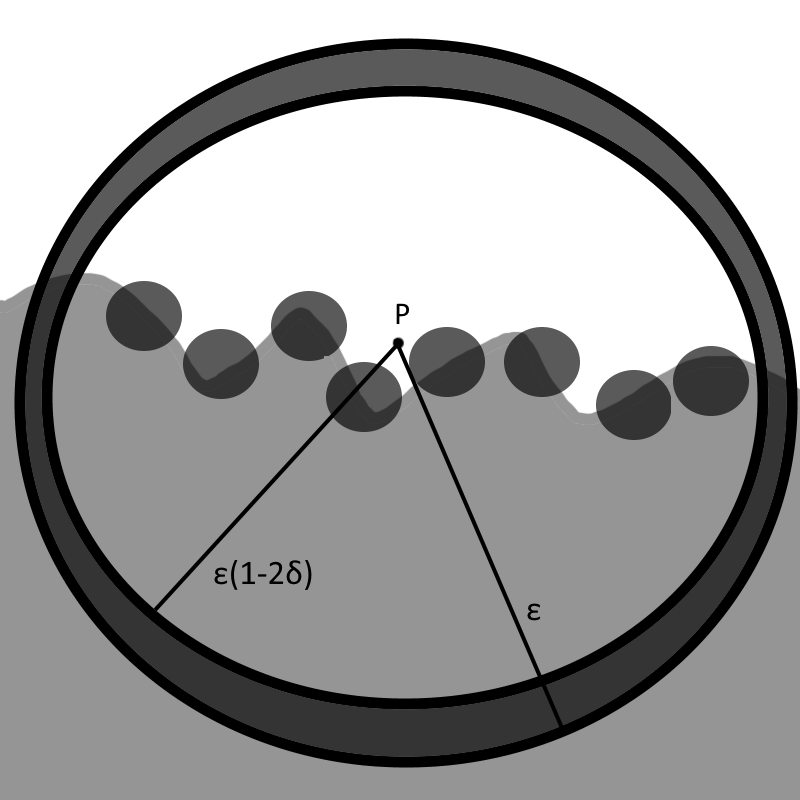
\includegraphics[width=0.4\textwidth]{covering lemma}
% \end{figure}

\begin{sublemma}\label{mollify sublemma}
If $n \geq 1$ then on $B_{1 - 2\sigma}$, for some $q > 0$,
$$(1_{V_n}(|\dif u| - Tu))_\varepsilon \lesssim_p \gamma^q (1_{V_n/2}|\dif u|)_\varepsilon.$$
\end{sublemma}

% \begin{sublemma}
% On $B_{1 - 2\sigma} \cap \{c\gamma^2 < \varphi < 1 - c\gamma^2\}$,
% $$(1_{V_0}(|\dif u| - Tu))_\varepsilon \lesssim_p \gamma |\dif u|_\varepsilon.$$
% \end{sublemma}
% \begin{proof}
% It follows from the definitions that for every $P \in B_\varepsilon$ and $Q \in V_0$, $\chi_\varepsilon(P - Q) \lesssim \varepsilon^{-d} \delta$,
% whence, by Proposition \ref{doubling dimension},
% \begin{align*}
% (1_{V_0}(|\dif u| - x\partial_zu))_\varepsilon &\lesssim \frac{\delta}{\varepsilon^d} \int_{B_\varepsilon} *|\dif u| \lesssim \frac{\delta}{\varepsilon}.
% \end{align*}
% Let $P \in B_\varepsilon$. Then by Lemma \ref{Giusti71}, there exists $c > 0$ such that if $\varphi \in (c\gamma^2, 1 - c\gamma^2)$, then there exists $Q \in \partial^* U$ such that $d(P, Q) < \varepsilon(1 - \gamma)$.
% If $d(Q, R) < \gamma\varepsilon/2$, then $d(P, R) < \varepsilon - \gamma\varepsilon/2$ and so $\chi_\varepsilon(P - R) \gtrsim \varepsilon^{-d}\gamma$ whenever $R \in B(Q, \gamma\varepsilon/2) =: W_0(P)$.
% We thus estimate
% $$\varepsilon^{-1} \gamma^{d - 1} \lesssim (1_{W_0(P)}|\dif u|)_\varepsilon \leq |\dif u|_\varepsilon$$
% and hence we obtain
% $$(1_{V_0}(|\dif u| - x\partial_zu))_\varepsilon(P) \lesssim \delta \gamma^{1 - d} |\dif u|_\varepsilon$$
% uniformly in $P$. Since $\delta = \gamma^d$, the claim holds.
% \end{proof}

Since the sets $V_n$ are approximately disjoint, as long as we chose $q < 1$, we can sum over $n$ to obtain
\begin{equation}\label{claim on main mollifier lemma 2}
|\dif \varphi| - T\varphi \lesssim_p \gamma^q |\dif u|_\varepsilon = \gamma^q |\dif \varphi|.
\end{equation}
which implies (\ref{claim on main mollifier lemma}). Thus we may fix
$$P \in \partial^* U \cap \{r < \sigma\} \cap \{\varphi \in (f(\gamma), 1 - f(\gamma)),$$
and observe that by (\ref{claim on main mollifier lemma 2}) we have $T\varphi(P) \gtrsim |\dif \varphi|(P)$.
Thus, in particular,
$$T\varphi(P) \gtrsim \int_{\{r < \varepsilon\}} *\chi_\varepsilon \cdot |\dif u|(P - \cdot) > 0$$
since $P \in \partial^* U$.
By Lemma \ref{Giusti71}, it follows that $\varphi$ is a $C^1$ submersion near $P$, so its level sets are $C^1$ near $P$.
\end{proof}

\begin{proof}[Proof of Sublemma \ref{mollify sublemma}]
It follows from the definitions, and an approximation of the metric $g$ by the euclidean metric that for every $n \geq 1$, $P \in B_{1 - 2\sigma}$, $\rho \in (0, 1)$, and $Q \in \rho V_n$, if $\gamma$ is small enough then
\begin{equation}\label{approximation of mollifier 2}
\varepsilon^{-d}\left(1 - \frac{4\delta}{\rho} - (1 + o_\varepsilon(1))\frac{\dist(P, Q_n)}{\varepsilon}\right) \lesssim \chi_\varepsilon(P - Q) \lesssim \varepsilon^{-d}\left(1 + \frac{4\delta}{\rho} - (1 + o_\varepsilon(1))\frac{\dist(P, Q_n)}{\varepsilon}\right).
\end{equation}
By (\ref{approximation of mollifier 2}), we can bound
\begin{align*}
(1_{V_n}(|\dif u| - Tu))_\varepsilon(P) &\lesssim F_n(P) \cdot \int_{V_n} *(|\dif u| - Tu), \\
F_n(P) &:= \frac{1}{\varepsilon^d}\left(1 + 4\delta - \frac{|P - Q_n|}{\varepsilon}\right).
\end{align*}
If $\gamma$ is chosen small enough, then $\sigma > 2\delta\varepsilon$ and so if we set $W_n = B(Q_n, \sigma)$ and apply Proposition \ref{Monotonicity Formula},
\begin{align*}
\int_{V_n} *(|\dif u| - Tu) &\leq (2\delta\varepsilon)^{d - 1}
 \left[\sigma^{1 - d}\int_{W_n} *(|\dif u| - Tu) + \sigma^{1 - d}\int_{W_n} *Tu - (2\delta\varepsilon)^{1 - d}\int_{V_n} *Tu\right]\\
 &=: (2\delta\varepsilon)^{d - 1} (I + J - K).
\end{align*}
To bound $I$ we use (\ref{hypothesis on main mollifier lemma}):
$$I = \sigma^{1 - d}\int_{W_n} *(|\dif u| - Tu) \leq \gamma^{\frac{1 - d}{2(d - 1)} + 1} = \gamma^{1/2}.$$
By Proposition \ref{sharp monotonicity},
\begin{align*}
J - K &\lesssim \alpha \sqrt{e^{O(\sigma^2)}\sigma^{1 - d} \int_{W_n} *|\dif u| - (2\delta\varepsilon)^{1 - d} \int_{V_n} *|\dif u|} =: \alpha \sqrt L,\\
\alpha &:= 3 + (d - 1) \log \frac{\sigma}{2\delta\varepsilon}.
\end{align*}
Straight from the definitions we have
$$\alpha \lesssim 1 - \log \gamma.$$
To bound $L$ we decompose it as 
\begin{align*}
L &= O(\sigma^{3 - d}) \int_{W_n} *|\dif u| + \sigma^{1 - d} \int_{W_n} *(|\dif u| - Tu) + \sigma^{1 - d} \int_{W_n} *Tu - (2\delta\varepsilon)^{d - 1} \int_{V_n} *|\dif u|\\
&=: L_1 + L_2 + L_3 - L_4.
\end{align*}
From Proposition \ref{doubling dimension}, we have $L_1 \lesssim \sigma^2$, and from Proposition \ref{scalar curvature monotonicity}, $L_3 - L_4 \lesssim \sigma^2$.
Moreover from (\ref{hypothesis on main mollifier lemma}),
$$L_2 \lesssim \sigma^{1-d} \gamma = \gamma^{1 + (1 - d)/(2d - 1)}.$$
Then $1 + (1 - d)/(2d - 1) > 0$, so summing up $I + J - K$, there exists $q > 0$ such that
\begin{equation}\label{big bound 1}
1_{V_n}(|\dif u| - Tu))_\varepsilon \lesssim \delta^{d - 1} \varepsilon^{d - 1} \gamma^q F_n.
\end{equation}
Since $U$ has least perimeter, Proposition \ref{doubling dimension} implies that
$$\delta^{d - 1} \varepsilon^{d - 1} F_n \lesssim F_n \int_{V_n/2} *|\dif u|,$$
which is $\lesssim (1_{V_n/2}|\dif u|)_\varepsilon$ by (\ref{approximation of mollifier 2}).
\end{proof}

We now set up the proof of Proposition \ref{mollifier quant}.
After rescaling, we may fix a sequence $(u_n)$ of indicator functions of sets $(U_n)$ with least perimeter in $B_1$.
We define
$$\gamma_n := \int_{B_1} |\dif u_n| - x\partial_z u_n,$$
assume that $(\gamma_n) \in \ell^1$, and draw $t \in (0, 1)$ uniformly at random.
It now suffices to show that
\begin{align}
|\partial V_n \cap B_t| &\leq \eta(V_n, B_t) + o(\gamma_n), \label{mollifier prop1}\\
\left|\int_{B_t} |\dif u_n| - |\dif v_n| ~\vol\right| &\ll \gamma_n, \label{mollifier prop2}\\
\lim_{n \to \infty} g(\normal_{V_n}, X) &= 1, \label{mollifier prop4}
\end{align}
where the limit in (\ref{mollifier prop4}) is uniform, and for every vector field $Y$ with $|Y| \sim 1$ and $|\Div Y| \lesssim 1$,
\begin{equation}
\left|\int_{B_t} Y(u_n - v_n)~\vol\right| \lesssim \gamma_n^2. \label{mollifier prop3}
\end{equation}

Let $w_n = (u_n)_{\gamma_n^4}$, let $c$ be the constant given by Lemma \ref{main mollifier lemma}, and let $a_n = c\gamma_n$, $b_n = 1 - c\gamma_n$.
0By Proposition \ref{Coarea2},
$$\int_{B_t} |dw_n| ~\vol = \int_0^1 |\partial^* \{w_n > y\} \cap B_t| ~dy \geq \int_{a_n}^{b_n} |\partial^* \{w_n > y\} \cap B_t| ~dy.$$
By the mean value theorem, there exists $y_n \in (a_n, b_n)$ such that
\begin{equation}\label{MVT mollifier}
|\partial^* \{w_n > y_n\} \cap B_t| \leq \frac{1}{b_n - a_n} \int_{B_t} |dw_n| ~\vol.
\end{equation}
If set $V_n = \{w_n > y_n\}$, $v_n = 1_{V_n}$, then $V_n$ has $C^1$ boundary in $B_t$ by definition of $a_n, b_n$, and from (\ref{claim on main mollifier lemma}), the locally uniform convergence (\ref{mollifier prop4}) holds.

So it remains to show that (\ref{mollifier prop1}--\ref{mollifier prop3}) hold almost surely.
Towards this end we will later show that
\begin{align}
|\partial V_n \cap B_t| &\leq |\partial^* U_n \cap B_t| + o(\gamma_n), \label{approximation of surface area} \\
\int_{\partial B_t} |u_n - v_n| ~\vol_{\partial B_t} &\lesssim \gamma_n^2. \label{approximation of volume}
\end{align}
If (\ref{approximation of surface area}, \ref{approximation of volume}) are true,
then by (\ref{a priori estimate 3}, \ref{approximation of volume}),
$$|\partial^* U_n \cap B_t| \leq |\partial V_n \cap B_t| + o(\gamma_n)$$
so by (\ref{approximation of surface area}), (\ref{mollifier prop2}) holds.
From an integration by parts using the estimate $1/2 \leq g(Y, Y) \leq 2$, and (\ref{approximation of volume}),
\begin{align*}
\left|\int_\Omega Y(u_j - v_j) ~\vol\right|
&\leq \left|\int_{\partial \Omega} (u_j - v_j)g(Y, \normal) ~\vol_{\partial \Omega}\right| \\
&\lesssim \int_{\partial \Omega} |u_j - v_j| ~\vol_{\partial \Omega} \lesssim \gamma_n^2
\end{align*}
which gives (\ref{mollifier prop3}).
By the fact that $U_n$ has least perimeter, and (\ref{a priori estimate 1}, \ref{mollifier prop2}),
\begin{align*}
|\partial V_n \cap B_t| &\leq |\partial U_n \cap B_t| + o(\gamma_n) \\
&= \eta(U_n, B_t) + o(\gamma_n)\\
&\leq \eta(V_n, B_t) + \int_{\partial B_t} |u_n - v_n| ~\vol_{\partial B_t} + o(\gamma_n),
\end{align*}
so by (\ref{approximation of volume}), (\ref{mollifier prop1}) holds.

%%%%%%%%%%%%%%%%%%%%%%%%%%%%%%%%%%%%%%%%%%%%%%%%%%%%%%%%%%%%%%%%

\begin{proof}[Proof of (\ref{approximation of surface area})]
By Lemma \ref{Giusti72}, one has
\begin{equation}\label{Giusti 720a}
\limsup_{n \to \infty} \int_{B_t} |du_n| - |dw_n| ~\vol \leq \limsup_{n \to \infty} \int_{B_{t + \gamma_n^4} \setminus B_t} |du_n| ~\vol.
\end{equation}
If we define $\mu = \sum_n \gamma_n|du_n| ~\vol$, then $\mu(B_1) < \infty$, since $(\gamma_n) \in \ell^1$ and $|\partial^* U_n \cap B_1|$ is uniformly bounded (c.f. Proposition \ref{doubling dimension}).
The hypotheses of \cite[(7.20)]{Giusti77} are (\ref{Giusti 720a}) and the fact that $\mu$ is a finite Borel measure on $B_1$, and the conclusion is that almost surely,
\begin{equation}\label{Giusti 720b}
\limsup_{n \to \infty} \gamma_n^{-2} \int_{B_t} |dw_n| - |du_n| ~\vol \leq 0.
\end{equation}
From (\ref{MVT mollifier}, \ref{Giusti 720b}), one has (\ref{approximation of surface area}).
\end{proof}

\begin{proof}[Proof of (\ref{approximation of volume})]
Let
$$f_n(t) = \gamma_n^{-4} \int_{B_t} |u_n - w_n| ~\vol.$$
By Lemma \ref{Giusti72} and the fact that $U_j$ has least perimeter in $B_1$,
$$\limsup_{n \to \infty} f_n(t) \leq \limsup_{n \to \infty} \int_{B_1} |du_n| ~\vol \leq |\partial B_1|.$$
Moreover, $f_n$ is monotone.
This implies that almost surely, $f_n'(t)$ is uniformly bounded in $n$.
But
$$f_n'(t) = \gamma_n^{-4} \int_{\partial B_t} |u_n - w_n| ~\vol_{\partial B_t},$$
so
\begin{equation}\label{mollify cubic gamma}
\int_{\partial B_t} |u_n - w_n| ~\vol_{\partial B_t} \lesssim \gamma_n^4.
\end{equation}
We now set $z_n = \min(y_n, 1 - y_n)$ and estimate
\begin{align*}
\int_{\partial B_t} |u_n - v_n| ~\vol_{\partial B_t} &= |\partial B_t \cap U_n \Delta V_n| \\
&= |\partial B_t \cap V_n \setminus U_n| + |\partial B_t \cap U_n \setminus V_n| \\
&\leq \frac{y_n}{z_n} |\partial B_t \cap V_n \setminus U_n| + \frac{1 - y_n}{z_n} |\partial B_t \cap U_n \setminus V_n|.
\end{align*}
From definition of $V_n$, $w_n - u_n > y_n$ on $V_n \setminus U_n$ and $u_n - w_n > 1 - y_n$ on $U_n \setminus V_n$, so
\begin{align*}
\int_{\partial B_t} |u_n - v_n| ~\vol_{\partial B_t} &\leq z_n^{-1} \int_{\partial B_t \cap U_n \setminus V_n} |u_n - w_n| ~\vol_{\partial B_t} + z_n^{-1}\int_{\partial B_t \cap V_n \setminus U_n} |u_n - w_n| ~\vol_{\partial B_t} \\
&\leq z_n^{-1} \int_{\partial B_t} |u_n - w_n| ~\vol_{\partial B_t}.
\end{align*}
But
$$z_n^{-1} \leq \max(y_n^{-1}, (1 - y_n)^{-1}) \leq \max(a_n^{-1}, b_n^{-1}) \lesssim \gamma_n^{-2}$$
whence
$$\int_{\partial B_t} |u_n - v_n| ~\vol_{\partial B_t} \lesssim \gamma_n^{-2} \int_{\partial B_t} |u_n - w_n| ~\vol_{\partial B_t},$$
so by (\ref{mollify cubic gamma}), (\ref{approximation of volume}) holds.
\end{proof}
